\documentclass[tikz,border=10pt]{standalone}
\usepackage{amsmath}
\usepackage{amssymb}
\usetikzlibrary{calc, arrows.meta}

% Define colors to match a modern aesthetic while distinguishing vectors
\definecolor{vecorange}{HTML}{E65100} % Light
\definecolor{vecgreen}{HTML}{2E7D32}  % Reflection
\definecolor{vecblue}{HTML}{1565C0}   % View
\definecolor{vecdark}{HTML}{BDBDBD}   % Normal (Light Gray for visibility)
\definecolor{vecpurple}{HTML}{9C27B0} % Halfway
\definecolor{surfbg}{HTML}{9E9E9E}

\begin{document}
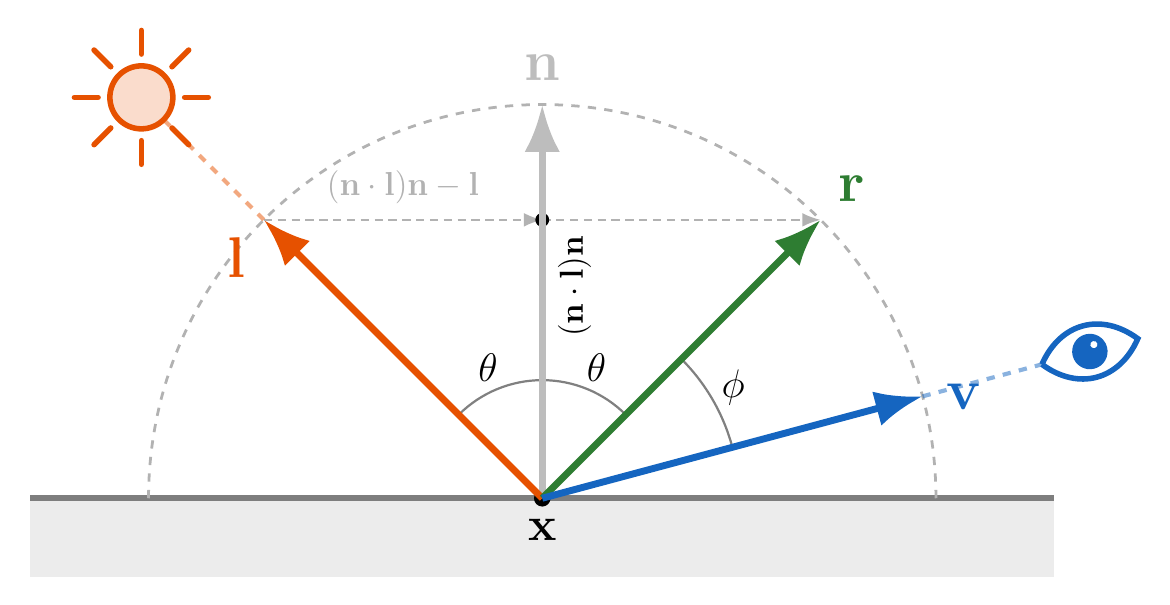
\begin{tikzpicture}[
    vec/.style={line width=2.5pt},
    >={Latex[length=6mm, width=4.5mm]}
]

% 1. Geometric parameters (Recalculated for perfect spacing)
\pgfmathsetmacro{\thetaAngle}{45}
\pgfmathsetmacro{\Langle}{90+\thetaAngle} % 135
\pgfmathsetmacro{\Rangle}{90-\thetaAngle} % 45
\pgfmathsetmacro{\Vangle}{15}
\pgfmathsetmacro{\phiAngle}{\Rangle-\Vangle} % 30
\pgfmathsetmacro{\Hangle}{(\Langle+\Vangle)/2} % 75 (Exactly halfway)

\pgfmathsetmacro{\vecLen}{5.0}
\pgfmathsetmacro{\SunDist}{7.2}
\pgfmathsetmacro{\EyeDist}{7.2}

\coordinate (O) at (0,0);
\coordinate (Ltip) at (\Langle:\vecLen);
\coordinate (Rtip) at (\Rangle:\vecLen);
\coordinate (Vtip) at (\Vangle:\vecLen);
\coordinate (Htip) at (\Hangle:\vecLen);
\coordinate (Ntip) at (90:\vecLen);
\coordinate (Nproj) at (0, {\vecLen*sin(\Langle)});

% 2. Surface Ground
\fill[surfbg!20] (-6.5, -1) rectangle (6.5, 0);
\draw[line width=2pt, surfbg!80!black] (-6.5, 0) -- (6.5, 0);

% 3. Origin Point (x)
\fill (O) circle (3pt);
\node[below=4pt, font=\LARGE] at (O) {$\mathbf{x}$};

% 4. Unit Hemisphere (To justify dot product scalar lengths)
\draw[dashed, gray!60, line width=1pt] (\vecLen, 0) arc (0:180:\vecLen);

% 5. Angles
% n to l (theta)
\draw[gray, thick] (90:1.5) arc (90:\Langle:1.5);
\node[font=\Large] at (112.5:1.8) {$\theta$};

% n to r (theta)
\draw[gray, thick] (90:1.5) arc (90:\Rangle:1.5);
\node[font=\Large] at (67.5:1.8) {$\theta$};

% r to v (phi)
\draw[gray, thick] (\Rangle:2.5) arc (\Rangle:\Vangle:2.5);
\node[font=\Large] at (30:2.8) {$\phi$};

% 6. Vector Construction Lines
% First step: l vector projected distance
\draw[-Latex, gray!60, densely dashed, thick] (Ltip) -- (Nproj) node[midway, above=2pt, font=\large] {$(\mathbf{n} \cdot \mathbf{l})\mathbf{n} - \mathbf{l}$};

% Second step: Completing the parallelogram to r
\draw[-Latex, gray!60, densely dashed, thick] (Nproj) -- (Rtip);

% Projection Point on Normal
\fill (Nproj) circle (2.5pt);
\node[right=4pt, below=24pt, font=\large, inner sep=1.5pt, rounded corners=2pt, rotate=90] at (0, {\vecLen*sin(\Langle)}) {$(\mathbf{n} \cdot \mathbf{l})\mathbf{n}$};

% 7. Main Shading Vectors
\draw[->, vec, vecdark] (O) -- (Ntip) node[above=4pt, font=\huge] {$\mathbf{n}$};
\draw[->, vec, vecorange] (O) -- (Ltip) node[below left=2pt, font=\huge] {$\mathbf{l}$};
\draw[->, vec, vecgreen] (O) -- (Rtip) node[above right=2pt, font=\huge] {$\mathbf{r}$};
\draw[->, vec, vecblue] (O) -- (Vtip) node[right=4pt, font=\huge] {$\mathbf{v}$};
% \draw[->, vec, vecpurple] (O) -- (Htip) node[above right=2pt, font=\huge] {$\mathbf{h}$};

% 8. Light Source (Sun) Context
\coordinate (SunPos) at (\Langle:\SunDist);
\draw[line width=1.5pt, vecorange, dashed, opacity=0.5] (Ltip) -- (SunPos);
\begin{scope}[shift={(SunPos)}]
    \fill[vecorange!20] (0,0) circle (0.4);
    \draw[vecorange, line width=2pt] (0,0) circle (0.4);
    \foreach \a in {0, 45, ..., 315} {
        \draw[vecorange, line width=2pt, line cap=round] (\a:0.55) -- (\a:0.85);
    }
\end{scope}

% 9. Viewer (Eye) Context
\coordinate (EyePos) at (\Vangle:\EyeDist);
\draw[line width=1.5pt, vecblue, dashed, opacity=0.5] (Vtip) -- (EyePos);
\begin{scope}[shift={(EyePos)}, rotate=\Vangle, scale=0.9]
    \fill[white] (0,0) ellipse (0.7 and 0.4);
    \draw[line width=2pt, vecblue] (-0.7,0) .. controls (-0.3,0.5) and (0.3,0.5) .. (0.7,0)
                            .. controls (0.3,-0.5) and (-0.3,-0.5) .. (-0.7,0);
    \fill[vecblue] (0,0) circle (0.25);
    \fill[white] (0.08,0.08) circle (0.05); % eye glint
\end{scope}

\end{tikzpicture}
\end{document}